\documentclass[12pt]{article}


\usepackage[a4paper, margin=2.4cm]{geometry}


\usepackage{graphicx}
\usepackage{float}
\usepackage{hyperref}



\begin{document}


\begin{abstract}
\centering
The simplified template cross section method for collecting data about the Higgs is considered as a potential target for machine learning methods, for identification and classification of events from the diphoton decay. This combination is designed to be applied to upcoming LHC data, to measure the properties of the Higgs more accurately and look for deviation from the Standard Model. Deep learning, a new machine learning technique, is analysed as a potential upgrade to the methods being used currently. 
\end{abstract}

\section*{Introduction}
In 2012, the ATLAS \cite{atlasann} and CMS \cite{cmsannouncement} collaborations at the Large Hadron Collider (LHC) announced the discovery of a new particle believed to be the Higgs boson. This was the culmination of over 50 years of theoretical and experimental work to complete the Standard Model of Particle Physics (SM), the mathematical theory which predicted the existence and properties of many new particles \cite{smpredictions}. However, whether this particle discovered was the SM Higgs needed testing, leading to an ongoing study of its properties and couplings to other particles. Any discrepancy found would give evidence for new physics, and possibly help to explain some of the gaps in current theories.

The Higgs boson is a scalar (spin 0) boson with even parity. At the LHC, the primary production mode is gluon fusion, followed by vector boson fusion (VBF) \cite{higgsproduction}. 

\begin{figure}[H]
\centering
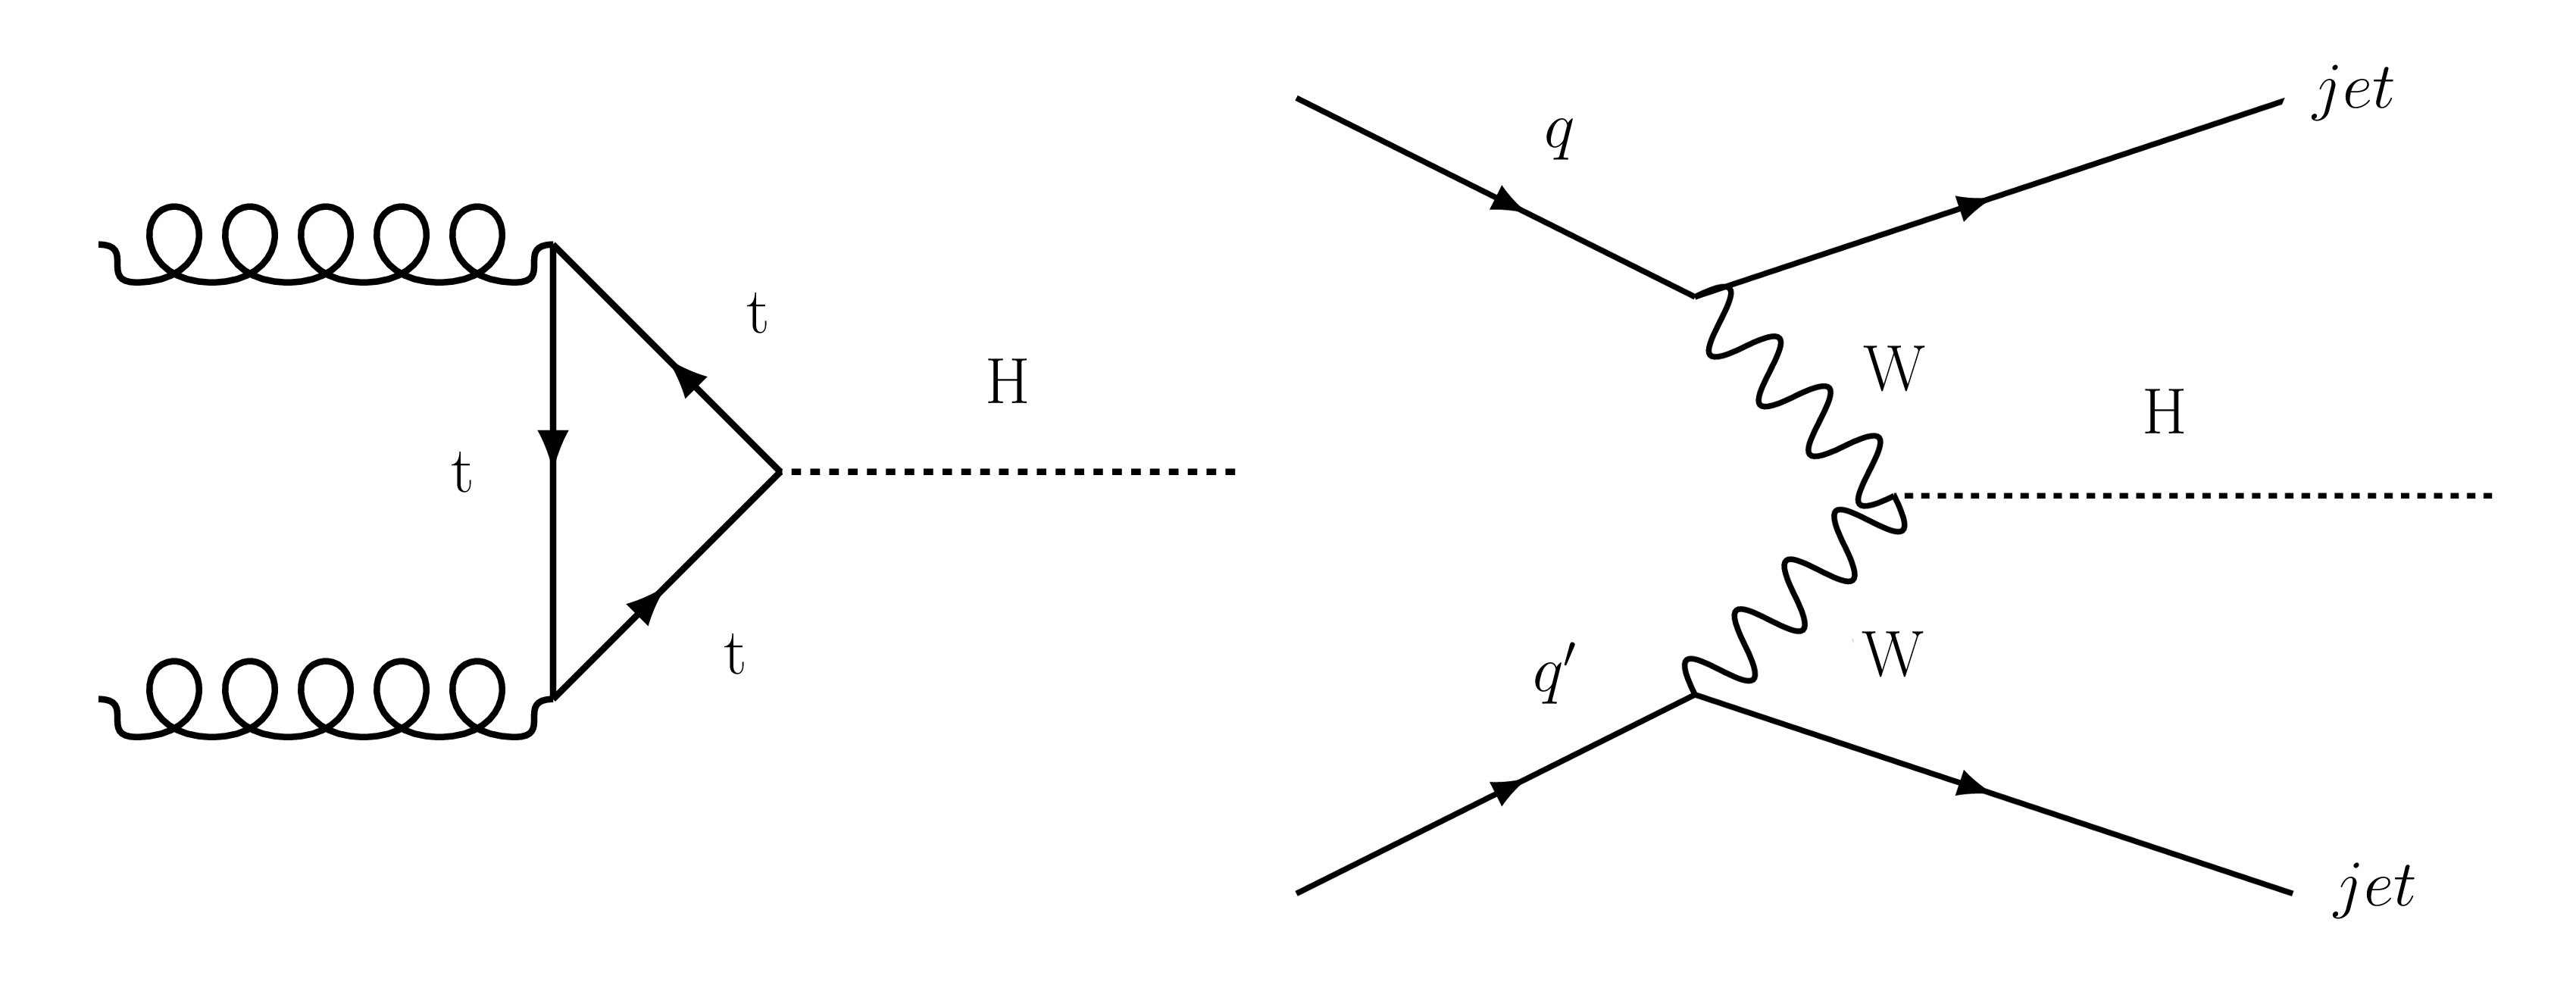
\includegraphics[width=12cm]{form.png}
\caption{Feynman diagrams for gluon fusion (left) and vector boson fusion (right). The forward jets from VBF can be used to identify it compared to other modes \cite{feynmanmaker}.}
	\label{form}
\end{figure}

Alternative production modes include associated production with a W boson and the recently observed associated production with top quarks \cite{tth}. These modes are all individually useful as they have distinct signatures and can be used to probe the couplings of the Higgs with the different particles involved. 

The decay modes include decays into vector bosons, two tau leptons, two b quarks and two photons \cite{gluinotheory1}, which is the decay mode considered in this project. Despite having a relatively small cross-section \cite{cmsannouncement}, the diphoton mode has the advantage of being a very clean mode, since the photons do not produce jets. It also has very good mass resolution, as the invariant mass of the photons gives a sharp peak \cite{seezdiphoton}. Additionally, the diphoton decay is interesting since it proceeds via a loop process, due to the photon being massless and therefore having no direct coupling to the Higgs. This makes the decay mode more sensitive to interference effects from potential new particles \cite{cmsanalysis1}. 

\begin{figure}[H]
\centering
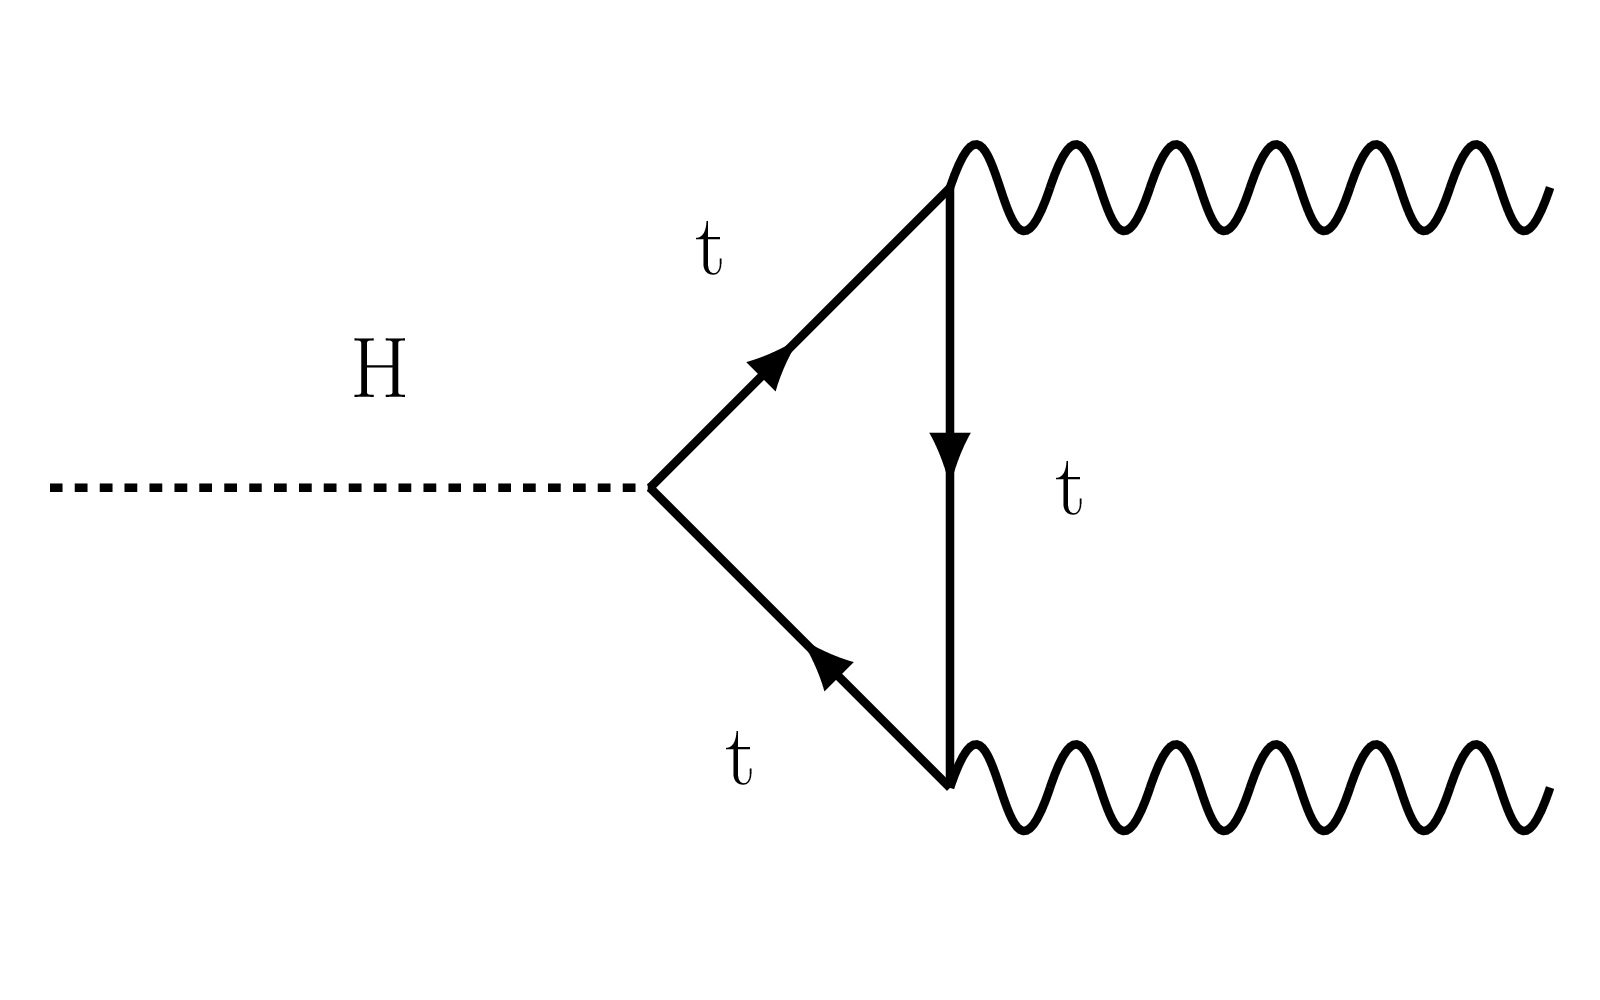
\includegraphics[width=6cm]{decay.png}
\caption{A possible Feynman diagram for the diphoton decay via a top quark loop. Another possibiliy is a W boson loop \cite{feynmanmaker}.}
	\label{decay}
\end{figure}

So far, all results seen are consistent with the SM, and the Higgs's spin-0 and even parity properties have been confirmed \cite{cmsupdate2} \cite{parity2}. For each of the production and decay modes, a variable $\sigma$/$\sigma_{SM}$ is defined to test compatibility with the SM, referred to as $\mu$. This is expected to be close to 1, and indeed all measurements of it so far have been consistent with expectations \cite{atlasann}\cite{cmsupdate2}.

Simplified template cross sections are a method for interpreting data first used in LHC Run 1, where the cross sections of each production mode are separated and split into multiple `bins', mutually exclusive areas of phase space, in order to systematically reduce the theory dependence of results. This can help reduce the theoretical uncertainties associated with measured values, as well as removing the dependencies on the underlying physics model being used, something that is particularly helpful when looking for BSM physics. 

With the large volumes of data the LHC produces, finding a way to make this data more manageable is important. In recent years, machine learning has increased in popularity as a tool to do this. These algorithms can be trained to identify event signatures from backgrounds based on a set of criteria. 

The aim of this project is to analyse and improve the current machine learning techniques being used at CMS in H$\rightarrow \gamma\gamma$, in order to increase its usage for event selection and categorisation into the `bins' defined by the simplified template cross section method, as well as potentially looking at how the binning choices could be expanded for future data analyses. This will allow better measurement of the Higgs boson's properties, allowing for more detailed tests of the SM Higgs and further probing for BSM physics in the diphoton decay. 

\section*{Background material}

\subsection*{Theory}

Spontaneous symmetry breaking is where a system in the ground state does not have the same symmetry as the Lagrangian that describes it. This is observed in nature, but the physical origin of the breaking remains a mystery. Including this broken symmetry and quantising the fields predicts the existence of `gauge' bosons such as the W and Z. However, this requires all bosons to be massless due to Goldstone's theorem \cite{higgstheory}, which presents a problem as the weak force is known to have a very short range so any mediator particles are required to be massive.

A solution was provided by Schwinger \cite{theory1}, Englert and Brout \cite{theory2}, Higgs \cite{higgstheory} and Guralnik, Hagen and Kibble \cite{theory3}. Their insights were that introducing a new scalar field to break the symmetry allowed the W and Z bosons to acquire mass by `absorbing' three of the four degrees of freedom in the field \cite{theory4}. The Higgs boson is the fourth degree of freedom, and the particle seen is the excitation of this new scalar field. This theory does not predict the mass of the Higgs boson, rather it is a parameter that if known allows all the expected coupling strengths to be predicted. 

It was later observed by Weinburg that via a Yukawa interaction (an interaction between a scalar field like the Higgs field and a Dirac field, which describes the behaviour of fermions) this would also give mass to fermions \cite{lepmass}. Combining the unified electroweak model with this new information produces what is now referred to as the Standard Model of Particle Physics. 


\subsection*{Methodology of the diphoton channel}
The expected signature of a H $\rightarrow \gamma\gamma$ decay is a narrow peak above the background found in the mass spectrum of the two photon system \cite{sethpresentation}. The observation of this has two main stages - the identification of the photons, and the measurement of their properties in order to reconstruct the decay. In the first stage, energy deposits in the electromagnetic calorimeter (ECAL) consistent with a photon are looked for. If an event has two of these, they will be analysed further to make sure that the particles are photons, since electrons and fragments from hadron jets such as $\pi^{0}$ will leave similar deposits \cite{recon}. To do this, a set of criteria called `Photon identification' are developed. To find the invariant mass of the photon pair, angles are needed so the point of decay needs to be reconstructed (as the photons don't leave any deposits in the inner part of the detector). This is difficult, since it can only be done statistically, and any errors in the vertex position will increase the width of the mass peak \cite{review1}. Another uncertainty which could increase the width are imperfect energy measurements in the ECAL, but these can be corrected for \cite{cmslimits}. Finally, additional criteria designed to differentiate between a Higgs decay and a background decay are applied to the data. The main background in this decay channel is QCD production of two photons, and is irreducible \cite{atlaslimits}. 

Thus, as well as working on upgrading the LHC and the detectors themselves, the methods of photon identification, reconstruction and signal/background identification have needed improvements with each data run \cite{cms13tev1}. With improvements to the LHC itself, an additional challenge is presented by the increasing data volumes, which has led to greater need for better data processing methods such as machine learning.


\subsection*{Machine learning methods}

Generally, the aim for any machine learning algorithm being used on LHC data is to cut away as much uninteresting data as possible. This could be immediately discarding bad quality events, or identifying particles based on detector deposits and separating this from expected backgrounds. The pattern recognition abilities of machine learning algorithms appear to be an efficient way to do this. These can be trained in two different ways; aided, where the training data is labelled to show what the features mean, and unaided, where the training data is unlabelled and the algorithm is left to make its own decisions. In particle physics, aided data sets are usually used, created by running simulations of the expected interactions in the detector \cite{mlreview}. 

Boosted decision trees (BDTs) are the most common method used currently \cite{ml7}. Here, each input variable is a `node', and the algorithm makes multiple cuts until some predefined end point is reached. The cuts are across multiple variables at once, and are chosen to maximise the change in some classifying variable, for example the signal-to-background ratio of a sample. Each data point is then classified as `signal' or 'background'. One problem with this method is that small statistical fluctuations in the training data can have a large impact. The solution to this is to use `boosting', where multiple decision trees are combined to reduce the errors and increase the overall stability \cite{ml8}. BDTs have been used successfully in experiments such as MiniBooNE \cite{ml2}, and are good at handling large data inputs, but even with the boosting are still not massively robust and can have issues with overfitting, where the tree created is specialised to the training data and doesn't work with real data as well \cite{ml1}. 

Both CMS and ATLAS have used BDTs in their analyses in a variety of different ways. For example, using a BDT to identify tau leptons in decays compared to electrons and jets has been implemented in ATLAS, with tests confirming the expected score distributions when run on different sets of simulated data \cite{ml4}. Similarly, ATLAS has also tested b tagging using BDTs \cite{ml5}. CMS made extensive use of BDTs during Run 1, using them for photon identification, uncertainty estimation and photon energy correction \cite{ml6}. Using a BDT allowed the photons to be classified by signal purity, allowing an additional analysis to be done on a smaller sample of data. The impact of this was estimated to be equal to collecting 50$\%$ more data \cite{mlreview}. These successes show machine learning in general is a useful tool in high energy physics.

In recent years, the improvements in BDTs for LHC data have started to slow down, leading to a search for alternatives \cite{ml9}. One class of algorithms that has received much interest recently is Deep Learning, which differs from `shallow' methods by teaching itself how to spot the features in the data rather than being taught. This makes them much more versatile than shallow methods and can lead to the algorithm itself finding better distinguishing features than the current set being used. It can also work with a larger set of criteria compared to current methods, however the training does take longer and is still prone to overfitting \cite{ml12}. 

A study testing the possible effectiveness attempted to identify the signatures of exotic particles using a deep neural network, and found that it out-performed both BDT and neural network shallow methods even when the shallow methods were explicitly given criteria based on expected physics \cite{ml9}. Despite a few cases where the data quality became the limiting factor rather than the algorithm \cite{ml3}, deep learning has had many successes. ATLAS tested one for b-tagging, which reduced the misidentification by a factor of 4. The method combined with a BDT for faster training still reduced this by a factor of 3 \cite{ml10}. It has also been used successfully to identify the tau Higgs decay against the background \cite{ml11}. These results show that deep learning has promise for event classification, making it a very useful tool should one need to categorise events according to specific criteria. 


\subsection*{Simplified template cross sections}
Simplified template cross sections involve measuring the cross section of each production mode divided into regions defined by their kinematic variables. This is done directly rather than measuring the signal strength, removing the theory dependence on the efficiency of the Higgs decay and acceptance limits, which are usually estimated computationally \cite{stxs1}. Since the signal strength is calculated from a combination of the cross-section and these theoretical estimates, measuring just the cross section gives more accurate data to work with while still making it possible to calculate the signal strength in the old way.

The bins are chosen differently for each production mode, allowing them to be designed for the expected signatures and topologies. The boundaries of the phase space regions are chosen to minimise extrapolation and maximise the sensitivity of the measurements. They are also chosen to minimise the number of bins required, and to allow potential BSM effects to be identified clearly \cite{stxs4}. Splitting the data in this way gives more information about the Higgs while having the benefit of combined decay mode information, allowing the testing of theoretical models in more detail than before. 

There are three `stages' of subdivision, designed to be measured in succession and updated based on measurements made before it. At stage 0, each production mode has one bin, with some modes like VBF and associated Higgs production grouped together due to similarities in signature. Stage 1 separates these bins further by kinematic properties. The aim is for all analyses to reach the specific subdivisions defined. Stage 2 divides the stage 1 bins, but before these can be defined stage 1 information is needed \cite{stxs3}. 


While the stage 0 bins are similar to Run 1 categorisations, so far only ATLAS has managed to measure stage 1 bins at $\sqrt{13}$ TeV. The diphoton section is split into 29 categories, using kinematic variables such as transverse momentum, number of jets, missing energy and invariant mass. Due to not having enough data sensitivity, the regions were merged into 9 phase space regions. All of the regions were found to be compatible with the Standard Model. The precision in measurement of the diphoton cross section was improved, but still limited by the data uncertainties. Thus, it was concluded that better quality data is needed to allow greater stage 1 splitting \cite{stxs2}. 
 

\section*{Conclusion}
In conclusion, while the discovery of the Higgs and subsequent confirmation of its properties have been a great triumph for modern physics, there are still many things in and beyond the Standard Model that are not understood. The LHC is aiming to answer these questions in the future, but with upgrades come new challenges to deal with the increases in data volume. A promising way to do this is with machine learning, which can be used to identify events and other interesting patterns in data from the background, but the currently used methods in Particle Physics are starting to struggle so new approaches are needed. Simultaneously, the methods used for data analysis can be improved, and simplified template cross sections look like a good method for increasing the quality and usefulness of experimental measurements, as well as flagging up any BSM physics that is being seen at the LHC.


\bibliography{bv1}{}
\bibliographystyle{unsrt}
\end{document}